\documentclass[a4paper, 12pt]{article}
\usepackage{erics-preamble}

\title{Erics derivata}
\author{Eric Fridén}
\date{\today}

\begin{document}

\doublespacing
\maketitle

\section{Deriveringsregler}

\subsection{Vad är derivata?}

Att ``derivera'' är att ta en funktion $f(x)$ och göra om den till en ny funktion som visar \emph{förändringshastigheten} av den första!

Den nya funktionen kallas \emph{derivatan} av $f(x)$. Den skrivs $f'(x)$ som uttalas `` f-prim av x''.

\begin{figure}[h]
    \centering
    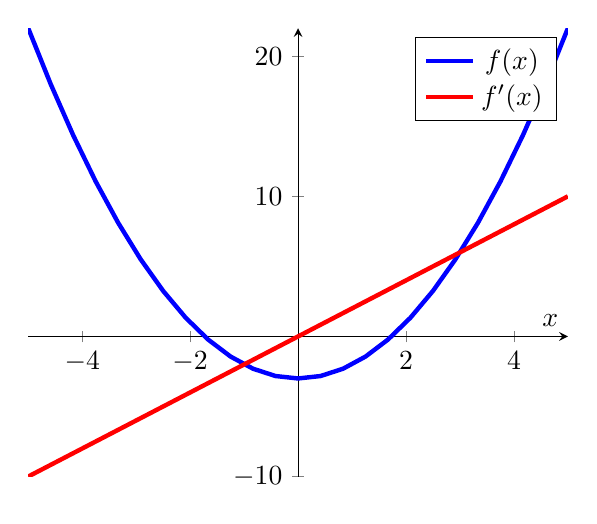
\begin{tikzpicture}
        \begin{axis}[
            axis lines = center,
            xlabel = \(x\)
        ]
        \addplot[blue, ultra thick] {x*x-3};
        \addlegendentry{$f(x)$}
        \addplot[red,  ultra thick] {2*x};
        \addlegendentry{$f'(x)$}
        \end{axis}
    \end{tikzpicture}
    \caption{När funktionen i blått pekar neråt (sett från vänster till höger) är derivatan i rött negativ. Ju mer positiv (uppåt) lutning grafen till funktionen har, desto mer positiv blir derivatan.}
    \label{fig:1}
\end{figure}

I figur \ref{fig:1} så är $f(x) = x^2 - 3$ och $f'(x) = 2x$. Målet med det här kapitlet är att lära oss reglerna vi följer när vi tar reda på derivatan av en funktion.


\subsection{Derivatan av $x^n$}

\begin{regel}
    \label{reg:x^n}
    \[f(x) = x^n \imp f'(x) = nx^{n-1}\]
\end{regel}

\begin{exempel}
    Vad är derivatan av $x^3$?\\
    Svar: $f'(x) = 3\cdot x^{3-1} = 3x^2$
\end{exempel}


\begin{exempel}
    Vad är derivatan av $f(x) = 1$\\
    Svar: $f(x) = x^0 \imp f'(x) = 0 \cdot \left [ \text{spelar ingen roll vad som kommer här}\right] = 0$
\end{exempel}

\begin{uppgifter}
    \label{upp:x^n}
    Derivera följande funktioner:
    \begin{multicols}{3}
        \begin{enumerate}
            \item $f(x) = x^4 \\ f'(x) \ans$
            \item $g(x) = 1 \\ g'(x) \ans$
            \item $h(x) = x^{27} \\ h'(x) \ans$
        \end{enumerate}
    \end{multicols}
\end{uppgifter}

\subsection{Derivatan av polynom}

\begin{regel}
    \label{reg:kxn}
    \[f(x) = kx^n \imp f'(x) = knx^{n-1}\]
\end{regel}
Som du kanske märker i räkneregel \ref*{reg:kxn} så ''hände'' det inget med $k$:et. Det är en generell regel för all derivata -- en siffra multiplicerad med en funktion finns kvar efter att funktionen deriverats. Vi kan formulera den generella regeln så här:

\begin{regel}
    \label{reg:kf(x)}
    \[ f(x) = k g(x) \imp f'(x) = k g'(x) \]
\end{regel}

\begin{exempel}
    Vad är derivatan av $3x^2$? \\ Svar: $f'(x) = 3\cdot 2x^{2-1} = 6x$
\end{exempel}

\begin{exempel}
    Vad är derivatan av $3$? \\ Svar: $f(x) = 3 \cdot x^0 \imp f'(x) = 3 \cdot 0 = 0$
\end{exempel}

\begin{uppgifter}
    \label{upp:kx^n}
    Derivera följande funktioner:
    \begin{multicols}{3}
        \begin{enumerate}
            \item $f(x) = 3x^4 \\ f'(x) \ans$
            \item $g(x) = 4 \\ g'(x) \ans$
            \item $h(x) = 2x \\ h'(x) \ans$
        \end{enumerate}
    \end{multicols}
\end{uppgifter}

Vi behöver en till regel för att kunna derivera alla polynom -- vi behöver veta hur vi hanterar funktioner med plustecken i. Som tur är så fungerar det på enklast tänkbara sätt, vi deriverar bara varje term för sig.

\begin{exempel}
    \label{ex:3x2}
    Vad är derivatan av $3x^2 + x^3$? \\ Svar: $f'(x) = 6x + 3x^2$
\end{exempel}

Du kanske ser mönstret utifrån exemplet, här är iallafall den generella regeln:

\begin{regel}
    \label{reg:sum}
    \[ f(x) = g(x) + h(x) \imp f'(x) = g'(x) + h'(x) \] 
\end{regel}

Kolla igen på exempel \ref*{ex:3x2} här ovanför och se att du är med på hur det funkar innan du gör övningsuppgifterna här under.

\begin{uppgifter}
    \label{upp:f+g}
    Derivera följande funktioner:
    \begin{multicols}{3}
        \begin{enumerate}
            \item $f(x) = 3x^4 + 1 \\ f'(x) \ans$
            \item $g(x) = 4x^2 + 3x \\ g'(x) \ans$
            \item $h(x) = 2x^{27} - 3x^3 + x \\ h'(x) \ans$
        \end{enumerate}
    \end{multicols}
\end{uppgifter}

\subsection{Icke-naturliga tal i exponenten}
En sak jag inte nämnde när vi introducerade räkneregel \ref{reg:x^n} på sidan \pageref{reg:x^n} var att $n$ INTE måste vara ett positivt heltal --- exakt samma regel gäller om exponenten är -2 eller $\frac 13$ eller $2,35$.

\begin{exempel}
    \label{ex:x^1/3}
    Vad är derivatan av $f(x) = x^{-2} + x^{\frac 13} + x^{2,35}$ ?

    Svar:
    \[ f'(x) = (-2)x^{-2-1} + \frac 13 x^{\frac 13 - 1} + 2,35 x^{2,35-1} = -2x^{-3} + \dfrac{x^{-\frac 23}}{3} + 2,35x^{1,35} \]
\end{exempel}

I de här övningsuppgifterna så får du träna på liknande saker som dyker upp i exempel \ref{ex:x^1/3}. Om du fastnar så kom ihåg att titta på potensreglerna i appendix \ref{app:pot} på sidan \pageref{app:pot}.


\begin{uppgifter}
    \label{upp:x^1/3}
    Derivera följande funktioner:
    \begin{multicols}{3}
        \begin{enumerate}
            \item $f(x) = \sqrt{x} \\ f'(x) \ans$
            \item $g(x) = \dfrac 1{x} + \dfrac 1{x^2} \\ g'(x) \ans$
            \item $h(x) = 4x^{0,5} \\ h'(x) \ans$
        \end{enumerate}
    \end{multicols}
\end{uppgifter}

\subsection{Derivatan av $a^x$}
Nu ska vi utvidga till derivator av funktioner där $x$ finns i exponenten, en grupp av funktioner som kallas \emph{exponentialfunktioner.}

Vi har följande regel som gäller för ett speciellt värde, när siffran i basen är $e \approx 2,77$. För en förklaring för vad $e$ är och var regeln kommer från, se Appendix \ref*{app:e} på sidan \pageref*{app:e}.

\begin{regel}
    \[f(x) = e^x \imp f'(x) = e^x \]
\end{regel}

\begin{uppgifter} 
    \label{upp:e^x}
    Derivera följande funktioner: \\(kom ihåg räkneregel \ref*{reg:kf(x)} på sidan \pageref*{reg:kf(x)}, och räkneregel \ref*{reg:sum} på sidan \pageref*{reg:sum}).
    \begin{multicols}{3}
        \begin{enumerate}
            \item $f(x) = e^x \\ f'(x) \ans$
            \item $g(x) = 3e^x \\ g'(x) \ans$
            \item $h(x) = 2e^x + x^2 \\ h'(x) \ans$
        \end{enumerate}
    \end{multicols}
\end{uppgifter}


\begin{regel}
    \label{reg:e^kx}
    \[ f(x) = e^{kx} \imp f'(x) = ke^{kx} \]
\end{regel}


\begin{exempel}
    Vad är derivatan av $f(x) = e^{3x}$? \\
    Svar: $f'(x) = 3e^{3x}$
\end{exempel}


\begin{exempel}
    Vad är derivatan av $f(x) = \dfrac 1{e^x}$? \\
    Lösning: Vi börjar med att skriva om $f(x)$ med hjälp av potensregler (se Appendix \ref*{app:pot} på sidan \pageref*{app:pot}). 
    \[ \frac 1{e^x} = e^{-x} = e^{(-1)x} \]
    Nu kan vi använda räkneregel \ref*{reg:e^kx}. \\
    Svar: $f'(x) = (-1)\cdot e^{(-1)x} = -e^{-x} = -\dfrac 1{e^x}$
\end{exempel}


\begin{uppgifter}
    \label{upp:e^kx}
    Derivera följande funktioner:
    \begin{multicols}{3}
        \begin{enumerate}
            \item $f(x) = \dfrac{1}{e^{-3x}} \\ f'(x) \ans$
            \item $g(x) = e^{5x} \\ g'(x) \ans$
            \item $h(x) = 2e^x + \dfrac 1{e^x} - e^{-2x} \\ h'(x) \ans$
        \end{enumerate}
    \end{multicols}
\end{uppgifter}

\subsubsection{Funktionen $a^x$}
Om du tittar på figur \ref*{fig:2^x} på sidan \pageref*{fig:2^x} och figur \ref*{fig:4^x} på sidan \pageref*{fig:4^x} i Appendix \ref*{app:e} så ser du att derivatan får en faktor framför sig, 1,4 i ena fallet och 0,7 i det andra. Den faktorn är värdet av funktionen $\ln(2)$ för $f(x) = 2^x$ och $\ln(4)$ för $f(x) = 4^x$. Funktionen $\ln (x)$ kallas för den \emph{naturliga logaritmen} och beskrivs i mer detalj i Appendix \ref*{app:e}


\begin{regel}
    \label{reg:a^x}
    \[f(x) = a^x \imp f'(x) = \ln (a) a^x \]
\end{regel}


\begin{exempel}
    \label{ex:a^x}
    Vad är derivatan till $3^x$?
    Svar: $f'(x) = \ln (3) 3^x$
\end{exempel}

Vi räknar väldigt sällan ut vad ett tal som $\ln(3)$ blir i decimalform --- om vi inte absolut behöver så är det enklast att låta det stå som det är.

Vi har en till regel för detta som liknar regel \ref*{reg:e^kx} på sidan \pageref*{reg:e^kx}:

\begin{regel}
    \label{reg:a^kx}
    \[f(x) = a^{kx} \imp f'(x) = k\ln(a)a^{kx}\]
\end{regel}


\begin{exempel}
    Vad är derivatan av $f(x) = \dfrac 2{4^{2x}}$?
    
    Lösning: Vi börjar med att skriva om $f(x)$ med hjälp av potensregler (se Appendix \ref*{app:pot} på sidan \pageref*{app:pot}).
    \[\dfrac{2}{4^{2x}} = 2\dfrac{1}{4^{2x}} = 2\cdot 4^{-2x} = 2\cdot 4^{(-2)x}\]

    Nu kan vi använda räkneregel \ref*{reg:a^kx}.

    Svar: $f'(x) = 2\cdot (-2) \cdot \ln(4) 4^{-2x} = - \dfrac {4\ln(4)} {4^{2x}}$
\end{exempel}

\begin{uppgifter}
    \label{upp:a^kx}
    Derivera följande funktioner:
    \begin{multicols}{3}
        \begin{enumerate}
            \item $f(x) = 3^x \\ f'(x) \ans$
            \item $g(x) = \dfrac{1}{2^{-3x}} \\ g'(x) \ans$
            \item $h(x) = 2\cdot 3^x + \dfrac 2{3^x} - \dfrac 2{3^{-x}} \\ h'(x) \ans$
        \end{enumerate}
    \end{multicols}
\end{uppgifter}

\newpage

\begin{blu}
    Derivera följande funktioner: (kom ihåg potensreglerna i Appendix \ref*{app:pot} på sidan \pageref*{app:pot})
    
    \begin{itemize}
        \begin{tabular}[b]{p{10em} p{20em}}
            \item $f(x) = x^2$  & \item[] $ f'(x) \ans $ \\
            \item $g(x) = \dfrac{1}{x^2} $ & \item[] $g'(x) \ans$ \\
            \item $h(x) = 2\cdot 3^x + 3x^2 $ & \item[] $h'(x) \ans$ \\
            \item $i(x) = 2^x $ & \item[] $i'(x) \ans$\\
            \item $j(x) = e^{-x} - e^x $ & \item[] $j'(x) \ans$\\
            \item $k(x) = \dfrac{4}{3x^2}-e^x + 3 $ & \item[] $k'(x) \ans$\\
            \item $l(x) = x^{13} - 13^x $ & \item[] $ l'(x) \ans$ \\
            \item $m(x) = \dfrac{2}{5\cdot 3^x} $ & \item[] $ m'(x) \ans$ \\
            \item $n(x) = \dfrac{x^5}{5} $ & \item[] $ n'(x) \ans$ \\
            \item $o(x) = e^{x-3} $ & \item[] $ o'(x) \ans$ \\
            \item $p(x) = \dfrac{2^{x+2}}{2^{2(x-2)}}$ & \item[] $ p'(x) \ans$ \\
        \end{tabular}
    
    \end{itemize}
    
\end{blu}


\newpage

\Huge{\textbf{Appendix}}
\normalsize
\appendix

\section{Konstanten $e$ och funktionen $e^x$} 
\label{app:e}
Vi börjar med att studera grafen till funktionen $2^x$.

\begin{figure}[h!]
    \centering
    
    \begin{mdframed}[backgroundcolor=gray!10]
        \centering
        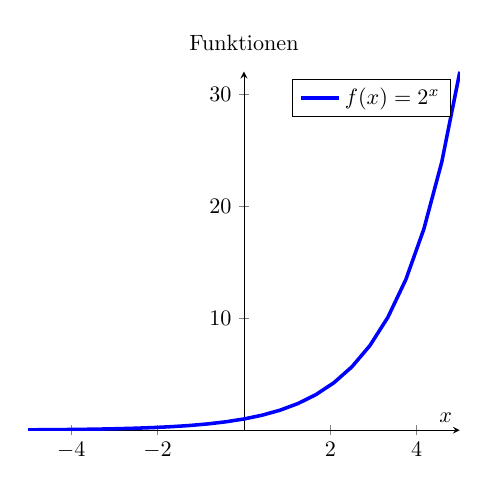
\begin{tikzpicture}[scale=.8]
            \begin{axis}[
                axis lines = center,
                xlabel = \(x\),
                ymin = 0,
                ymax = 32,
                title = Funktionen
            ]
            \addplot[blue, ultra thick] {2^x};
            \addlegendentry{$f(x) = 2^x$}
            \end{axis}
        \end{tikzpicture}
        \hskip 5em
        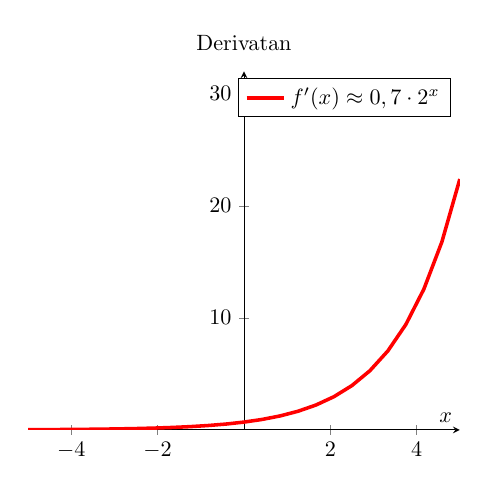
\begin{tikzpicture}[scale=.8]
            \begin{axis}[
                axis lines = center,
                xlabel = \(x\),
                ymin = 0,
                ymax = 32,
                title = Derivatan
            ]
            \addplot[red, ultra thick] {0.7*2^x};
            \addlegendentry{$f'(x) \approx 0,7\cdot 2^x$}
            \end{axis}
        \end{tikzpicture}  
        \caption{Exponentialfunktionen $f(x) = 2^x$ till vänster och funktionens derivata till höger.}
        \label{fig:2^x}
        
    \end{mdframed}
\end{figure}

Funktionen har en speciell egenskap: den lutar mer och mer brant ju större värdet blir. Det verkar som att \emph{derivatan} av $2^x$ ökar samtidigt som funktionen själv ökar, och att derivatans värde hela tiden är lite mindre än funktionens värde. Om vi testar med funktionen $f(x) = 4^x$ så får vi ett liknande samband --- men denna gång åt andra hållet, derivatan är lite större än funktionen.

\begin{figure}[h!]
    \centering
    \begin{mdframed}[backgroundcolor=gray!10]
        \centering
        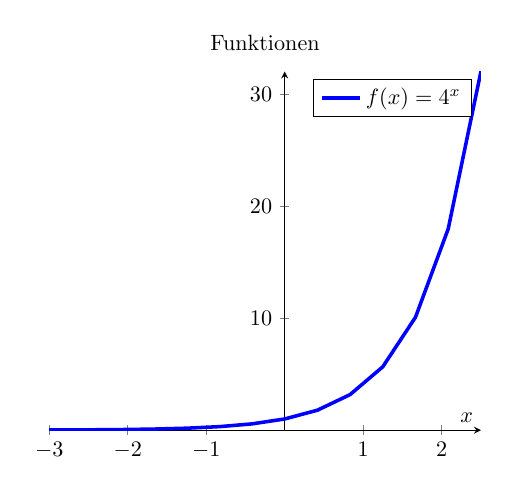
\begin{tikzpicture}[scale=.8]
            \begin{axis}[
                axis lines = center,
                xlabel = \(x\),
                ymin = 0,
                ymax = 32,
                xmin = -3,
                xmax = 2.5,
                title = Funktionen
            ]
            \addplot[blue, ultra thick] {4^x};
            \addlegendentry{$f(x) = 4^x$}
            \end{axis}
        \end{tikzpicture}
        \hskip 5em
        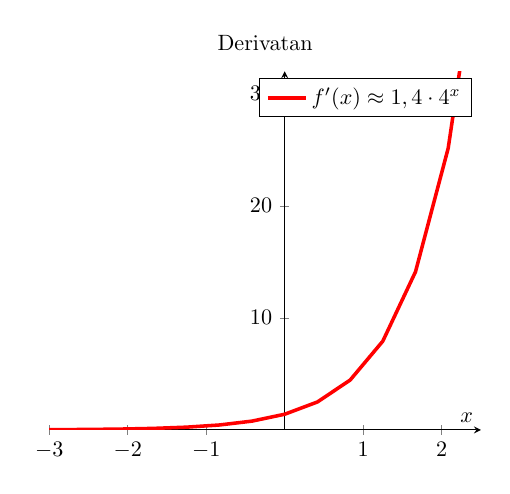
\begin{tikzpicture}[scale=.8]
            \begin{axis}[
                axis lines = center,
                xlabel = \(x\),
                ymin = 0,
                ymax = 32,
                xmin = -3,
                xmax = 2.5,
                title = Derivatan
            ]
            \addplot[red, ultra thick] {1.4*(4^x)};
            \addlegendentry{$f'(x) \approx 1,4\cdot 4^x$}
            \end{axis}
        \end{tikzpicture}
        \caption{Exponentialfunktionen $f(x) = 4^x$ till vänster och funktionens derivata till höger.}
        \label{fig:4^x}
    \end{mdframed}
\end{figure}

De två graferna liknar varandra --- men de är inte helt likadana. Någonstans mellan 2 och 4 finns ett tal som gör att $f(x)$ och $f'(x)$ är exakt likadana --- en funktion som är sin egen derivata. Det talet kallas $e$ och det är en konstant som är ungefär lika med 2,72.

\begin{figure}[h!]
    \centering
    \begin{mdframed}[backgroundcolor=gray!10]
        \centering
        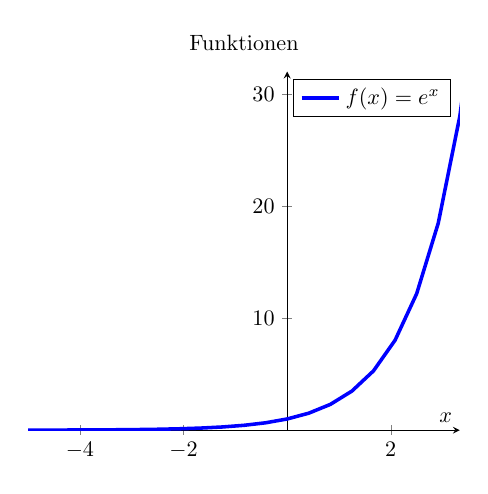
\begin{tikzpicture}[scale=.8]
            \begin{axis}[
                axis lines = center,
                xlabel = \(x\),
                ymin = 0,
                ymax = 32,
                title = Funktionen
            ]
            \addplot[blue, ultra thick] {e^x};
            \addlegendentry{$f(x) = e^x$}
            \end{axis}
        \end{tikzpicture}
        \hskip 5em
        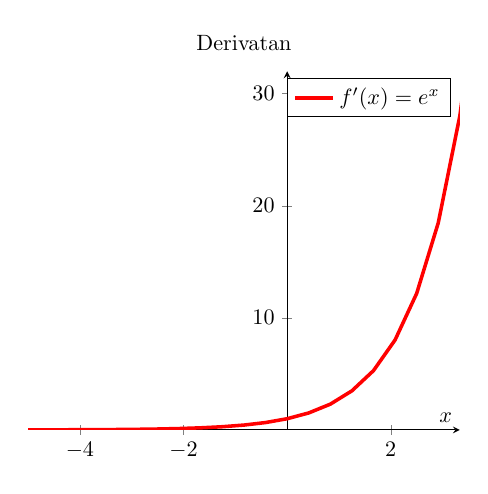
\begin{tikzpicture}[scale=.8]
            \begin{axis}[
                axis lines = center,
                xlabel = \(x\),
                ymin = 0,
                ymax = 32,
                title = Derivatan
            ]
            \addplot[red, ultra thick] {e^x};
            \addlegendentry{$f'(x) = e^x$}
            \end{axis}
        \end{tikzpicture}
        \caption{Exponentialfunktionen $f(x) = e^x$ till vänster och funktionens derivata till höger.}
        \label{fig:e^x}
    \end{mdframed}
\end{figure}

Vi har därmed hittat en funktion $f(x)$ som har den trevliga egenskapen att $f(x) = f'(x)$ --- vi kan formulera det som en väldigt användbar räkneregel:

\begin{regel}
    \label{reg:e^x}
    \[f(x) = e^x \imp f'(x) = e^x \]
\end{regel}

\subsection{Funktionen $\ln(x)$}

I det här häftet kommer vi att stöta på funktionen $\ln(x)$, \emph{den naturliga logaritmen}. Den definieras så här:


\begin{regel}
    \label{reg:lnx}
    \[ x = \ln(y) \imp e^x = y \]
\end{regel}

I fall när en funktion ett värde som t.ex. $\ln(3)$ som en del av sin lösning så räknar man generellt inte ut värdet av funktionen utan låter den stå som $\ln(3)$. Om man behöver räkna ut det så har alla datorer och de flesta miniräknare en $\ln$-funktion.

\newpage

\section{Potensregler}
\label{app:pot}
När man arbetar med derivata så dyker ofta potensfunktioner upp --- det är därför viktigt att ha bra koll på en del centrala potensregler.


\begin{regel}
    \[a^x \cdot a^y = a^{x+y} \]
    \[\left(a^x\right)^y = a^{xy}\]
    \[a^{-x} = \dfrac 1{a^x}\]
    \[a^{\frac 1n} = \sqrt[n]a\]
\end{regel}

Här följer exempel på hur potensreglerna kan dyka upp i resten av häftet.


\begin{exempel}
    Funktionen $f(x) = \dfrac1{e^x}$ kan inte deriveras med vanliga deriveringsregler --- men med hjälp av potensreglerna kan vi skriva om det:

    \[\dfrac1{e^x} = e^{-x} = e^{(-1)\cdot x}\]

    $f(x) = e^{(-1)\cdot x}$ kan deriveras med regel \ref*{reg:e^kx} på sidan \pageref*{reg:e^kx}.
\end{exempel}

\begin{exempel}
    Funktionen $f(x) = \dfrac {5^x}{5^{2x}}$ kan inte deriveras med vanliga deriveringsregler --- men med hjälp av potensreglerna kan vi skriva om det:

    \[\dfrac {5^x}{5^{2x}} = 5^x \dfrac 1{5^{2x}} = 5^x 5^{-2x} = 5^{x+(-2x)} = 5^{-x} = 5^{(-1)x}\]

    $f(x) = 5^{(-1)x}$ kan deriveras med regel \ref*{reg:a^kx} på sidan \pageref*{reg:a^kx}.

\end{exempel}

\begin{exempel}
    Funktionen $f(x) = e^{x+2}$ kan inte deriveras med vanliga deriveringsregler --- men med hjälp av potensreglerna kan vi skriva om det:

    \[e^{x+2} = e^xe^2 = e^2e^x\]

    $f(x) = e^2e^x$ kan deriveras med regel \ref*{reg:e^x} på sidan \pageref*{reg:e^x} och \ref*{reg:kf(x)} på sidan \pageref*{reg:kf(x)}.

\end{exempel}

\newpage
\section{Facit till övningsuppgifter}


\begin{facit}
    \begin{multicols}{3}
        \begin{enumerate}
            \item $f'(x) = 4x^3$
            \item $g'(x) = 0$
            \item $h'(x) = 27x^{26}$
        \end{enumerate}
    \end{multicols}
\end{facit}

\begin{facit}
    \begin{multicols}{3}
        \begin{enumerate}
            \item $f'(x) = 12x^3$
            \item $g'(x) = 0$
            \item $h'(x) = 2$
        \end{enumerate}
    \end{multicols}
\end{facit}

\begin{facit}
    \begin{multicols}{3}
        \begin{enumerate}
            \item $f'(x) = 12x^3$
            \item $g'(x) = 8x + 3$
            \item $h'(x) = 54x^{26} - 9x^2 + 1$
        \end{enumerate}
    \end{multicols}
\end{facit}


\begin{facit}
    \begin{multicols}{3}
        \begin{enumerate}
            \item $f'(x) = e^x$
            \item $g'(x) = 3e^x$
            \item $h'(x) = 2e^x + 2x$
        \end{enumerate}
    \end{multicols}
\end{facit}

\begin{facit}
    \begin{multicols}{3}
        \begin{enumerate}
            \item $f'(x) = \dfrac{3}{e^{-3x}}$
            \item $g'(x) = 5e^x$
            \item $h'(x) = 2e^x - \dfrac 1{e^x} + 2e^{-2x}$
        \end{enumerate}
    \end{multicols}
\end{facit}

\begin{facit}
    \begin{multicols}{3}
        \begin{enumerate}
            \item $f'(x) = \ln (3) 3^x$
            \item $g'(x) = \dfrac{3\ln (2)}{2^{-3x}}$
            \item $h'(x) = 2 \ln (3) 3^x - \dfrac{2\ln (3)}{3^x} - \dfrac {2\ln (3)}{3^{-x}}$
        \end{enumerate}
    \end{multicols}
\end{facit}

\newpage
\section{Facit blandade uppgifter}

\begin{blufacit}
    \begin{itemize}
        \item $f'(x) = 2x$
        \item $g'(x) = -\dfrac{2}{x^3}$
        \item $h'(x) = 2 \ln(3) + 6x$
        \item $i'(x) = \ln(2) 2^x$
        \item $j'(x) = -e^{-x}- e^x$
        \item $k'(x) = -\dfrac{8}{3x^3}-e^x$
        \item $l'(x) = 13x^{12} - \ln(13)13^x$
        \item $m'(x) = -\dfrac{2\ln(3)}{5\cdot 3^x}$
        \item $n'(x) = x^4$
        \item $o'(x) = e^{x-3}$
        \item $p'(x) = - \dfrac{2^6}{2^x}$
    \end{itemize}
\end{blufacit}

\end{document}